\subsection{Experimentation}

In diesem Unterkapitel werden verschiedene R-Pakete, welche Funktionen für Topic Modeling-Methoden bereitstellen, ausprobiert. Die meisten dieser Pakete werden in \cite{Wiedemann2022-tm-R} angeführt.

Als Datenquelle für die Modelle und Algorithmen wird \textbf{Projekt Gutenberg} herangezogen, ein Online-Archiv für historische Werke. Projekt Gutenberg stellt ein R-Paket zur Verfügung, wessen Verwendung in der Auflistung \ref{list:code-gutenbergr-inst} angeführt wird \cite{gutenbergr}.

\begin{listing}
    \begin{code}{R}
        install.packages("gutenbergr")
        library(gutenbergr)
    \end{code}
    \caption{Installation und Verwendung vom R-Paket "gutenbergr"}
    \label{list:code-gutenbergr-inst}
\end{listing}

Eine Zusammenfassung der wichtigsten Funktionen \cite{gutenbergr}:
\begin{itemize}
    \item Die Funktion \codeinline{R}{gutenberg_works()} gibt eine Liste aller Werke zurück. In der Klammer lassen sich als Parameter Filter wie \codeinline{R}{author=="XY"}, \codeinline{R}{title=="YX"} und \codeinline{R}{gutenberg_id==1234} einsetzen.
    \item \codeinline{R}{gutenberg_works()} gibt unter anderem eine \codeinline{R}{gutenberg_id} der Bücher zurück. Diese verwendet man in der Funktion \codeinline{R}{gutenberg_downloads()}. Diese Funktion kann mehrere IDs sowie sowie Metadaten als Parameter übernehmen, zum Beispiel:
    \\\codeinline{R}{gutenberg_download(c(568, 1204), meta_fields="author")}
\end{itemize}

Die Codezeilen aus der Auflistung \ref{list:code-poe} laden den Text aller Werke vom Author Edgar Allan Poe herunter und werden von allen Modellen verwendet.

\begin{listing}
    \begin{code}{R}
        ## using necessary packages
        library(gutenbergr)
        ## retrieving data from gutenberg
        search <- gutenberg_works(author=="Poe, Edgar Allan")$gutenberg_id
        poe_data <- gutenberg_download(search)$text
    \end{code}
    \caption{Codezeilen zum Download aller Werke von E.A. Poe}
    \label{list:code-poe}
\end{listing}


\subsubsection{Paket \codeinline{R}{textmineR}}

Das Paket \textbf{textmineR} ist einer der modernsten Pakete, welche LDA unterstützen \cite[288]{Wiedemann2022-tm-R}.

Weiters unterstützt es die Modelle LSA und CTM. In Folge werden einfache Prototypen erstellt, für welche man die Datenverarbeitung und deren Einfachheit des Pakets sowie den Output des Modells analysiert.

Das erste Beispiel bzw. Experiment vom Paket \codeinline{R}{textmineR} zeigt die Verwendung mit \textbf{LDA}. Der Code ist in der Auflistung \ref{list:code-textmeineR-lda} angeführt.

Das Ergebnis der letzten Funktion \codeinline{R}{SummarizeTopics(poe_lda)} ist in Abbildung \ref{fig:res-lda-textmineR} zu sehen. An sich tut es das, was es tun soll: Den zehn Topics wurden Wörter zugeordnet. 

Es gibt sogar Daten wie \codeinline{R}{prevalence} und \codeinline{R}{coherence}, welche für Analysezwecke des Modells selbst verwendet werden können. Es gibt jedoch zwei Dinge, die möglicherweise störend sind.

Einerseits wird den Topics bereits ein Label gegeben. Der ganze Sinn dieser Arbeit besteht darin, dass Schüler selbst die Topics benennen. Das ist nicht allzu schlimm, da man diese Spalte entfernen kann.

Was störender ist sind die zwei Spalten mit den Topic-bezogenen Wörtern. Vor allem der Umstand, dass manche Wörter zweimal vorkommen, hilft nicht. In der Dokumentation des Pakets \codeinline{R}{textmineR} steht auch nichts darüber, selbst die Anzahl der Wörter zu setzen, welche angezeigt werden. Das macht dieses Paket ungeeignet für manche Anwendungen, zum Beispiel wenn es einen Slider gibt, mit dem man die Anzahl der Wörter pro Topic bestimmen möchte.

\begin{listing}
    \begin{code}{R}
        ## neccessary packages
        library(textmineR)
        library(stringr)
        ## removing all non-english letters and characters
        ### due to error it is necessary to remove any unknown characters
        poe_data_n <- str_remove_all(poe_data, "[^[\\da-zA-Z ]]")
        ## creating a document term matrix (dtm)
        poe_dtm <- CreateDtm(doc_vec = poe_data_n)
        ## fitting a lda-model with 100 samples of data and 10 topics
        set.seed(123)
        poe_lda <- FitLdaModel(dtm = poe_dtm[1:700,], k = 15, iterations = 250, burnin = 210)

        ergebnis_lda <- SummarizeTopics(poe_lda)
        ergebnis_lda
    \end{code}
    \caption{Anwendungsbeispiel von LDA im Paket textmineR}
    \label{list:code-textmeineR-lda}
\end{listing}

\begin{figure}
    \centering
    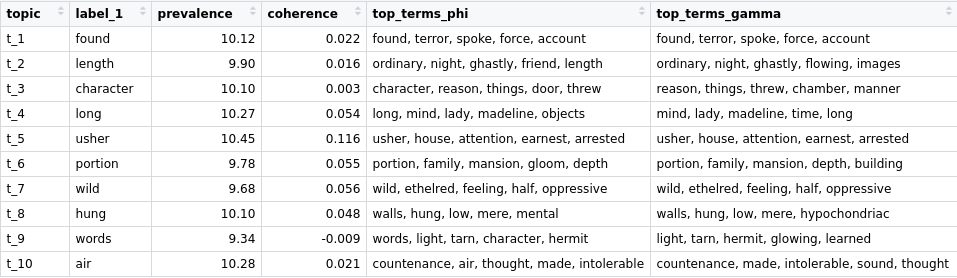
\includegraphics[scale=0.45]{images/dlengsteiner/ergebnis_textmineR_lda_n.png}
    \caption{Ergebnis von LDA (Paket \codeinline{R}{textmineR})}
    \label{fig:res-lda-textmineR}
\end{figure}

Das nächste Beispiel (Auflistung \ref{list:code-textmineR-lsa}) zeigt die Verwendung mit \textbf{LSA} (alle Variablen bis \codeinline{R}{poe_dtm} vom vorherigen Experiment wurden für dieses Experiment ebenfalls verwendet). 

Das zweite Problem von vorher ist hier verstärkt (siehe Abbildung \ref{fig:res-lsa-textmineR}). Es sind nämlich nicht nur ein paar Wörter in den top\_terms-Spalten doppelt veorhanden, sondern es sind alle Wörter betroffen. Je nach Anwendungsfall kann das zu einem Problem werden, vor allem Kombiniert mit der Tatsache, dass man die Anzahl der Wörter pro Topic nicht erhöhen kann.

\begin{listing}
\begin{code}{R}
    set.seed(1234)
    poe_lsa <- FitLsaModel(dtm = poe_dtm, k = 10)
    ergebnis_lsa <- SummarizeTopics(poe_lsa)
    ergebnis_lsa
\end{code}  
    \caption{Anwendungsbeispiel von LSA im Paket textmineR}
    \label{list:code-textmineR-lsa}
\end{listing}

\begin{figure}
    \centering
    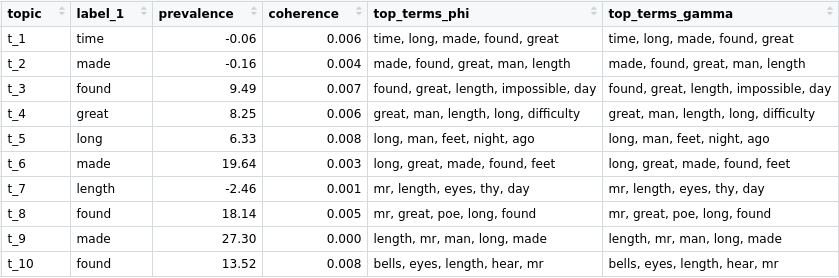
\includegraphics[scale=0.5]{images/dlengsteiner/ergebnis_textmineR_lsa.png}
    \caption{Ergebnis von LSA (Paket \codeinline{R}{textmineR})}
    \label{fig:res-lsa-textmineR}
\end{figure}

\newpage

\subsubsection{Paket \codeinline{R}{tm}}\label{sec:preprocessing-packages}

\paragraph{tm} The Package \codeinline{R}{tm}\cite{Feinerer2023-tm} is a powerfull package used in text mining. It is utilized in the pre-processing of textdata in this project. With a few commands, textdata is transformed into a DTM which can be used by the \codeinline{R}{topicmodels}-package to create a topic model (see \nameref{sec:topicmodels-package}).

As an example, listing \ref{list:code-tm-preprocessing} shows the pre-processing of the data \codeinline{R}{poe_data}. Depending on the size of the data this process may take a while, up to several minutes. The synergy with the package \codeinline{R}{topicmodels} makes this approach especially attractive, because said package is very competent in creating proper models without taking a long time.

\begin{listing}
\begin{code}{R}
# data has non-ASCII characters which have to be removed
poe_data$text <- str_remove_all(poe_data$text, "[^[\\da-zA-Z ]]")
# method DataframeSource() needs specifc column-names
colnames(poe_data) <- c("doc_id","text")
# creation of a usable corpus
corpus <- tm::VCorpus(DataframeSource(poe_data))
# Pre-processing process
## setting all words to lower-case
processedCorpus <- tm_map(corpus, content_transformer(tolower))
## removing stopwords (Erklärung notwendig!)
processedCorpus <- tm_map(processedCorpus, removeWords, stopwords())
## all punctuations are removed, except intra-word dashes
processedCorpus <- tm_map(processedCorpus, removePunctuation, preserve_intra_word_dashes = TRUE)
## remove numbers
processedCorpus <- tm_map(processedCorpus, removeNumbers)
## stems of english language are formed (Erklärung notwendig!)
processedCorpus <- tm_map(processedCorpus, stemDocument, language = "en")
## remove whitespaces (space, tabs, ...)
processedCorpus <- tm_map(processedCorpus, stripWhitespace)
# DocumentTermMatrix is created (Erklärung?). 
DTM <- tm::DocumentTermMatrix(processedCorpus, control = list(bounds = list(global = c(5, Inf))))
# After vocabulary pruning, empty rows exists which have to be removed
# before: 134322, after: 116465
sel_idx <- slam::row_sums(DTM) > 0
DTM <- DTM[sel_idx, ]
\end{code}  
    \caption{Preprocessing with the package tm}
    \label{list:code-tm-preprocessing}
\end{listing}


\paragraph{quanteda} 

\subsubsection{Package \codeinline{R}{topicmodels}}\label{sec:topicmodels-package}

This package supports LDA as well as CTM \cite{Grün2023-topicmodels}. The creation of both models only requires one method. 

Listing \ref{list:code-topicmodels-lda-ctm} shows both of these methods in acion, using the DTM created with the package \codeinline{R}{tm} (see \nameref{sec:preprocessing-packages}). The first argument is the Document Term Matrix provided by the package \codeinline{R}{tm}. The second argument is the amount of topics the model should generate. The third argument is the method used to train the model, in this case it is the Gibbs-sampling method (EXPLANATION REQUIRED). The fourth argument is used to control the execution of the command. In this case, the number of iterations is limited to 400 to reduce the time needed to fit the model (FURTHER EXPERIMENTATION AND COMPARISON BETWEEN MODELS REQUIRED).

\begin{listing}
    \begin{code}{R}
        topicModel_lda <- topicmodels::LDA(DTM, 40, method="Gibbs", control=list(iter=400))
    \end{code}
    \caption{Creation of LDA and CTM model with topicmodels}
    \label{list:code-topicmodels-lda-ctm}
\end{listing}


Unfortunately, visualizing these models in not very intuitive. This study will explore two methods of visualizing the topic models created by the package \codeinline{R}{topicmodels}. 

\paragraph{LDAvis} The first method is to use the Package \codeinline{R}{LDAvis}. It provides the function \codeinline{R}{serVis()} \cite[6]{Sievert2015-LDAvis}, which ouputs a visualisation of an LDA-model in a new browser window. The only parameter it needs to function is a JSON-String created by the function \codeinline{R}{createJSON()}. This method requires a lot of parameters \cite[2]{Sievert2015-LDAvis}. Listing \ref{list:code-topicmodels2LDAvis} shows a method to extract these parameters from the LDA-model and save them in the JSON-String.
\begin{listing}
    \begin{code}{R}
        topicmodels2LDAvis <- function(x, ...){
            post <- topicmodels::posterior(x)
            if (ncol(post[["topics"]]) < 3) stop("The model must contain > 2 topics")
                mat <- x@wordassignments
            LDAvis::createJSON(
                phi = post[["terms"]], 
                theta = post[["topics"]],
                vocab = colnames(post[["terms"]]),
                doc.length = slam::row_sums(mat, na.rm = TRUE),
                term.frequency = slam::col_sums(mat, na.rm = TRUE)
            )
        }
        LDAvis::serVis(topicmodels2LDAvis(topicModel_lda))
    \end{code}
    \caption{Method for saving necessary values into JSON-String created by \codeinline{R}{createJSON}}
    \label{list:code-topicmodels2LDAvis}
\end{listing}
This method has only one parameter \codeinline{R}{x}. This parameter must be a LDA-model from the package \codeinline{R}{topicmodels}. Line 2 of Listing \ref{list:code-topicmodels2LDAvis} uses the \codeinline{R}{posterior()}-function to extract the posterior probabilities from a model. The parameter \codeinline{R}{topicModel_lda} is the LDA-Model created in Listing \ref{list:code-topicmodels-lda-ctm}.

Running Line 13 will result in the output shown in Figure \ref{fig:output-ldavis}. This output is highly interactive. Each model can be individually selected, either by clicking on the corresponding circle or typing the number of the topic in the text input. The words at the right hand side of the screen will change accordingly. However, because this is a seperate browser window, integrating it into a shiny-app (see \nameref{sec:visualisierung}) could prove difficult. Also, there is the issue of a potential information-overload, especially for non-data scientists.
\begin{figure}
    \centering
    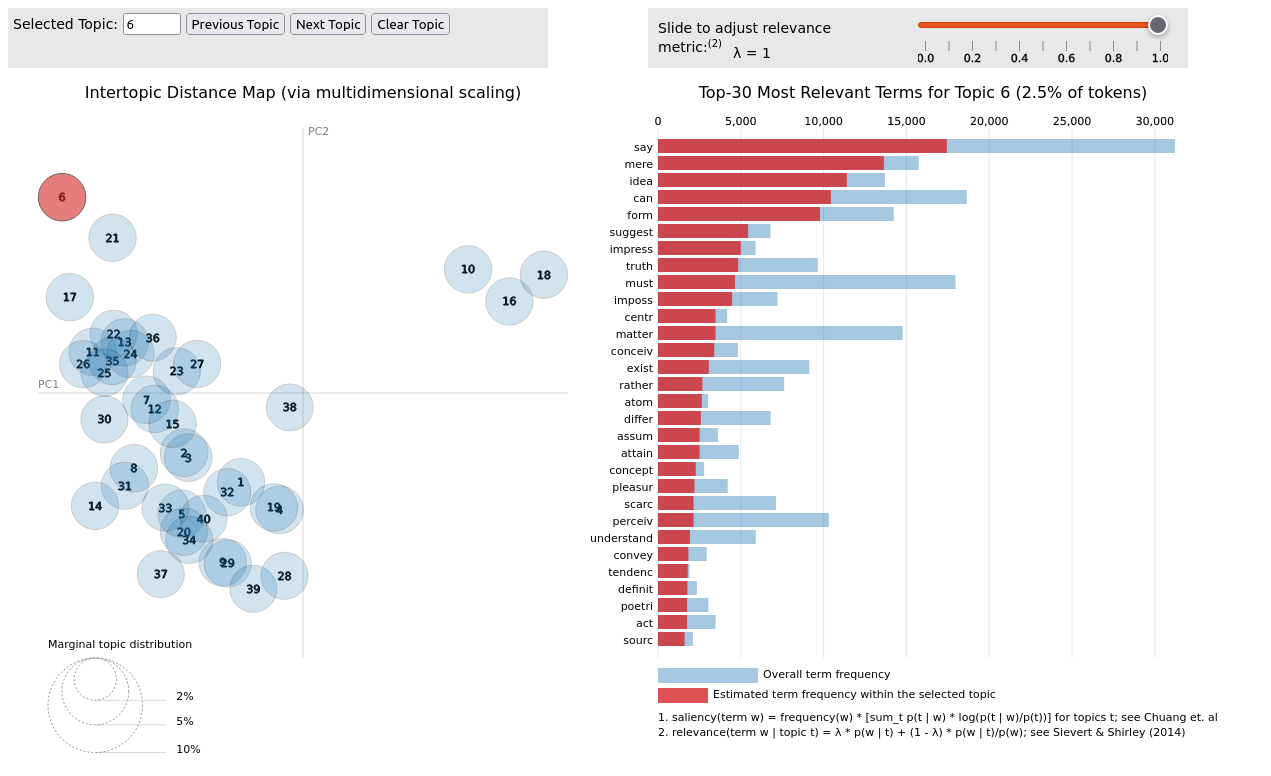
\includegraphics[scale=0.3]{images/dlengsteiner/output-LDAvis.png}
    \caption{Output of LDAvis in a browser window}
    \label{fig:output-ldavis}
\end{figure}


\paragraph{Custom visualisation} 


\subsubsection{Package \codeinline{R}{stm}}


